\section{Среда программирования распределённых мобильных приложений QReal:Ubiq}
\label{chapter:qRealUbiq}
Так же, как и QReal:Robots, QReal:Ubiq появилась из практической задачи, с которой к нам 
обратились представители индустрии --- программирование мобильных приложений в рамках архитектуры 
платформы Ubiq Mobile. В этом случае также имелась достаточно узкая предметная область, 
но приложения, которые требовалось разрабатывать, были гораздо ближе к типичным разрабатываемым 
промышленно приложениям, чем QReal:Robots, в частности, имели и нетривиальную логику, и 
пользовательский интерфейс. Поэтому данная задача была интересна как некоторая попытка 
заменить визуальным программированием программирование на текстовых языках для достаточно 
большого класса задач. Успешная реализация подобной технологии открыла бы возможность 
для создания целой серии технологий, направленных на различные платформы.

\subsection{Постановка задачи}
Платформа Ubiq Mobile~\cite{onossovski2009ubiq} предназначается для создания распределённых мобильных приложений со сложной серверной 
логикой, таких как бизнес-приложения, многопользовательские игры и т.д. Архитектурно 
платформа представляет собой сервер с выполняемыми на нём сервисами и набор мобильных 
клиентов, связанных с сервером по проприетарному протоколу. Клиенты могут работать 
на телефонах с очень маленькими возможностями, такими как устаревшие Java-телефоны, 
в этом случае используется тонкий клиент, который только отображает формируемое на 
сервере изображение пользовательского интерфейса и передаёт на сервер события нажатий 
на клавиши. Для более современных моделей возможна передача на клиент построенного 
на сервере дерева визуальных элементов управления, которые отображаются на телефоне 
средствами его операционной системы. Возможно также написание толстого клиента, реализующего 
часть бизнес-логики на телефоне. В любом случае, на сервере для каждого подключённого 
клиента создаётся отдельный поток, в котором и работает большая часть клиентской логики 
программы. Этот поток может общаться с потоками, относящимися к серверной части сервиса, 
таким образом достигается возможность взаимодействовать с серверной частью приложения и другими 
пользователями. Таким образом, сообщения между сервером и клиентом физически передаются 
между потоками, работающими на сервере, по каналу данных передаётся только результат 
обработки.

С точки зрения прикладного программиста процесс создания сервиса в Ubiq Mobile представляет 
собой программирование клиентского и серверных потоков как реализацию подклассов одного 
из классов платформы Ubiq Mobile. Требуется определить формат сообщений, которыми 
обмениваются клиент и сервер (в виде C\#-классов) и описать методы, реагирующие на 
приём сообщения на клиенте и на сервере. Также потребуется описать пользовательский 
интерфейс приложения, также в виде набора объектов на C\# (это делается в достаточно 
декларативном и удобном для текстового программирования стиле). Результат должен быть 
оформлен в виде C\#-библиотеки, собран вместе с библиотеками Ubiq Mobile, выложен в 
папку с исполняемым файлом сервера Ubiq Mobile и добавлен в его конфигурационный файл. 
Очевидно, что все подобные библиотеки имеют похожую структуру, и для их создания требуется 
выполнение повторяющихся действий, поэтому имеется возможность для автоматизации.

Авторы платформы Ubiq Mobile выбрали \ac{DSM}-платформу QReal для реализации технологии 
и набора визуальных языков, которые упростили бы разработку мобильных приложений под 
эту платформу. Целью совместной работы было создание на базе QReal технологии, позволявшей 
описывать в визуальном виде только изменяющуюся от приложения к приложению часть и 
генерировать по визуальной модели проект для среды разработки Visual Studio~\cite{visualStudio}, 
который был бы готов к сборке итоговой библиотеки, не требуя при этом ручных правок. 

Разработка была разделена на несколько этапов. Целью первого этапа было создание прототипа 
технологии, чтобы оценить применимость \ac{DSM}-подхода к этой задаче. Прототип должен 
был генерировать логику поведения клиентской части приложения, позволяющего осуществлять 
видеонаблюдение: веб-камера, подключённая к компьютеру, передаёт с определённой частотой 
кадры на сервер Ubiq Mobile, к серверу могут подключаться мобильные клиенты, которым 
перенаправляются кадры с камеры. И камер, и клиентов может быть несколько в один момент 
времени, клиент может указать, с какой камеры ему необходимо получать кадры 
(более подробно о мотивации и задаче этого примера было рассказано в докладе~\cite{terekhov2011ubiq}).
Пользовательский интерфейс клиентского приложения на этом этапе должен был описываться 
вручную. Задачи второго этапа включали в себя реализацию полноценной технологии, включающей 
в себя визуальное задание пользовательского интерфейса приложения. Ниже приводится 
подробное описание только первого этапа, поскольку работы по второму этапу ещё не 
закончены и ведутся со значительно меньшим участием автора данной диссертации.

\subsection{Визуальный язык QReal:Ubiq}
Фазы анализа применимости и анализа предметной области для данного \ac{DSM}-решения состояли 
в консультациях с авторами технологии Ubiq Mobile, выступавшими здесь в роли экспертов 
предметной области и в анализе существующих исходных кодов сервисов, написанных под 
эту платформу. В данном случае для выделения ключевых сущностей предметной области и 
создания языка был выбран подход <<от исходного кода>>, поскольку у авторов платформы 
уже имелся достаточно большой набор работающих примеров и понимание того, что хотелось 
бы автоматизировать.

В результате анализа исходного кода было принято решение разработать три различных 
визуальных языка, отвечавших двум основным областям вариативности создаваемых сервисов: 
описание структуры сообщений, которыми обмениваются клиент и сервер, и описание логики 
обработки сообщений на клиенте и на сервере. Третий визуальный язык был нужен для 
описания связи между различными диаграммами первых двух языков, диаграммы на нём 
служили чем-то вроде заголовка визуальной модели системы. 

Визуальные языки QReal:Ubiq состоят из следующих сущностей.
% TODO: Таблица?
\begin{enumerate}
	\item Мастер-диаграмма (Ubiq Master Diagram) описывает главный класс серверного 
		приложения и является по сути связью между остальными диаграммами системы. Эта 
		диаграмма должна содержать ровно один элемент Master Node, в котором описано, 
		откуда сервер получает сообщения и какие обработчики необходимо вызвать при их 
		получении. Такая диаграмма должна быть одна в проекте. Виды узлов на этой диаграмме таковы.
		\begin{enumerate}
			\item Constant --- константа, описанная внутри класса сервера. Имеет имя, тип 
				и значение. Может находиться только внутри Master Node.
			\item Field --- поле класса сервера. Имеет имя, тип, значение по умолчанию, 
				может быть отмечено как статическое. Может находиться только внутри Master Node.
			\item Handler --- описывает источник событий для сервера, имеет имя (которое 
				может принимать два значения: либо OnTcpIpMessage, что означает, что сервер 
				может обрабатывать сообщения, полученные по TCP-IP, либо OnMailBoxMessage, 
				что означает, что сервер может обрабатывать сообщения от другого процесса). 
				Может находиться только внутри Master Node. Каждый такой узел должен быть 
				связан с помощью провязки с диаграммой активностей, описывающей поведение 
				соответствующего обработчика.
			\item Master Diagram --- корневой узел диаграммы, все остальные узлы должны 
				быть вложены в него.
			\item Master Node --- описание класса серверной части приложения. Может содержать 
				в себе описания обработчиков событий, констант, полей, препроцессоров (узлы 
				Handler, Constant, Field, Preprocessor), имеет свойства <<имя>> (имя класса 
				сервера), initCode (произвольный код на C\#, генерирующийся в конструктор класса), 
				onTcpIpCloseHandler (произвольный код на C\#, выполняющийся при закрытии TCP-IP-соединения). 
				Может быть связан провязкой с диаграммами активностей, описывающими реализацию 
				вспомогательных функций, которые сгенерируются как методы этого класса.
			\item MasterDiagramComment --- комментарий.
			\item Preprocessor --- метод, вызываемый перед передачей сообщения обработчику, 
				предназначенный для преобразования сообщения перед передачей обработчику. 
				Должен быть провязан с диаграммой активностей, реализующей этот метод.
		\end{enumerate}
	\item Диаграмма структур данных (Ubiq Data Structures), на ней описывается класс 
		Message, предназначенный для обмена сообщениями между клиентом и сервером или 
		сервером и другими процессами, а также другие классы, служащие данными. Такая 
		диаграмма должна быть одна в проекте. Узлы на этой диаграмме таковы.
		\begin{enumerate}
			\item Comment --- комментарий.
			\item Custom Class --- произвольный класс, содержащий данные. Имеет свойство 
				<<имя>> (которое генерируется в имя класса), содержит в себе поля (элементы 
				типа Field).
			\item Data Structures Diagram --- сама диаграмма, корневой элемент.
			\item Enum Element --- элемент перечисления. Имеет имя и значение. Может находиться 
				в узлах Message Codes и Error Codes, будет сгенерирована как константа внутри 
				класса Message.
			\item Error Codes --- описание кодов ошибок, используемых в классе Message. 
				Должен быть один на диаграмме. Содержит в себе элементы Enum Element.
			\item Field --- произвольное поле класса Message или произвольного класса (может 
				лежать в Message Class или Custom Class), генерируется в свойство соответствующего 
				класса. Имеет имя (имя свойства), значение по умолчанию, тип, может быть сериализуемым 
				или несериализуемым.
			\item Message Class --- описание класса Message, должен быть один на диаграмме. 
				Содержит в себе только поля (элементы Field).
			\item Message Codes --- описание кодов сообщения, используемых в классе Message. 
				Должен быть один на диаграмме. Содержит в себе элементы Enum Element.
		\end{enumerate}
	\item Диаграмма активностей (Ubiq Activity Diagram). На таких диаграммах задаётся 
		поведение обработчика сообщений, метода, препроцессора и т.д. В модели их может 
		быть несколько (по числу обработчиков). Содержание несколько разнится в зависимости 
		от вида диаграммы --- диаграмма активностей для обработчика, диаграмма активностей 
		для препроцессора, вспомогательной функции. Диаграмма для обработчика обычно состоит 
		из нескольких цепочек операторов, начинающихся с узла HandlerStart, препроцессор 
		начинается с Initial Node, функция --- с Function Signature. Узлы, используемые 
		на всех видах диаграммы активностей, таковы.
		\begin{enumerate}
			\item Action --- действие, имеет свойство <<имя>>, которое должно содержать код 
				на C\#. Он будет без изменений скопирован в результат генерации.
			\item Activity Diagram --- сама диаграмма.
			\item Activity Final Node --- завершающий узел, означает конец цепочки операторов. 
				Полезен, например, для рисования пустой ветки else, в остальных случаях необязателен.
			\item Actual Parameter --- фактический параметр, передаваемый в функцию при вызове. 
				Имеет имя, которое должно быть C\#-кодом, подставляемым вместо параметра при 
				вызове функции, может содержаться только в узле Function Call.
			\item Comment --- комментарий.
			\item Control Flow --- направленная связь, означающая передачу управления от 
				оператора к оператору. Имеет свойство guard, используемое при генерации узлов 
				Decision Node.
			\item Decision Node --- оператор "if". Должен иметь ровно две исходящие связи, 
				ровно у одной из которых свойство guard не пусто. Обе ветки должны сходиться 
				либо на одном Merge Node, либо на одном Activity Final Node. Свойство guard 
				становится условием оператора if в сгенерированном коде.
			\item Formal Parameter --- формальный параметр, описываемый в заголовке вспомогательной 
				функции. Может содержаться только в узле Function Signature. Имеет имя и тип.
			\item Function Call --- вызов функции. Имеет имя, которое должно совпадать с 
				именем диаграммы активностей, реализующей вызываемую функцию. Содержит набор 
				параметров (узлов Actual Parameter), и максимум один узел Return Value, показывающий, 
				куда положить результат вызова функции.
			\item Function Signature --- описание вспомогательной функции, с него начинается 
				цепочка операторов диаграммы активностей для вспомогательной функции. Имеет имя 
				(должно совпадать с именем диаграммы) и тип возвращаемого значения. Может 
				содержать в себе формальные параметры (типа Formal Parameter).
			\item Handler Start --- начало обработчика сообщения. С него начинается цепочка 
				операторов на диаграмме активностей обработчика. Имеет имя, которое должно 
				совпадать с именем константы --- типа сообщения, описанного на диаграмме структур 
				данных.
			\item Initial Node --- начальный узел, с него начинается цепочка операторов 
				диаграммы активностей препроцессора.
			\item Merge Node --- точка слияния двух веток выполнения оператора if.
			\item Package --- вспомогательный узел, предназначенный для организации диаграмм 
				активностей в связанные блоки в логической модели. Семантической нагрузки не несёт.
			\item Return --- возврат значения из вспомогательной функции, генерируется в 
				оператор return C\#. Равносилен узлу Action с оператором return <возвращаемое значение>;
			\item Return Value --- указывает, куда положить возвращаемое функцией значение. 
				Может содержаться только в узле Function Call. Имеет имя (код на C\#, обычно 
				имя переменной) и тип. Если тип не пуст, генерируется объявление переменной 
				для хранения результата, если пуст, считается, что переменная уже объявлена.
		\end{enumerate}
\end{enumerate}

% TODO: Метамодель, примеры диаграмм

Как видно из описания, язык имеет гибридную структуру, то есть для задания программы 
активно используются и визуальные, и текстовые символы. При этом визуальная и текстовая 
части языка частично взаимозаменяемы --- язык позволяет не рисовать диаграмму обработчика 
сообщения, а написать весь код вручную в единственном блоке. В качестве текстовой 
части используется язык C\#, код на котором непосредственно генерируется в выходные 
файлы. Технология не имеет синтаксического анализатора языка C\#, поэтому не может 
выполнять никаких действий над содержимым блоков, даже синтаксические ошибки в коде 
будут обнаружены только после генерации. Язык задания логики обработчиков (диаграмма 
активностей) по сути представляет собой диаграмму активностей UML, модифицированную 
для того, чтобы отразить особенности Ubiq Mobile.

\subsection{Обсуждение}
Главный недостаток получившегося набора языков вытекает из выбранного способа анализа 
предметной области: визуальный язык слишком привязан к целевому коду, так что без 
достаточно хорошего владения технологией Ubiq Mobile или специальной подготовки создавать 
программы оказывается довольно сложно. Фактически, надо представлять, в какую часть программы 
будет сгенерирован тот или иной код, который пишется в узлах Action и различных других 
узлах, где допускается ввод кода на C\# вручную. Смысл некоторых свойств практически 
невозможно объяснить человеку, не знакомому детально с Ubiq Mobile (поэтому такие 
свойства опускались при описании языка). Кроме того, наличие в C\# переменных и полей 
классов делает возможным модификацию локального или даже глобального состояния из 
кода в узле Action обработчика, что приводит к неявным и никак не визуализируемым 
зависимостям по данным, на диаграммах визуализируется только поток исполнения. Фактически 
оказалось, что очень сложно писать код на C\# в элементах визуального языка, не смотря 
при этом в сгенерированный код. Кроме того, диаграммы активностей более громоздкие, 
чем код, который они призваны визуализировать, поэтому в них оказывается сложнее 
разобраться. Субъективный вывод, сделанный автором данной работы в ходе разработки 
модельного примера --- диаграммы активностей не оправдывают себя, проще и продуктивнее 
писать код обработчиков вручную.

Перечисленные недостатки являются проблемой для всех гибридных (текстографических) 
языков, в которых текстовая часть является кодом на целевом языке и не анализируется 
синтаксически самим \ac{DSM}-решением. В любом случае, пользователи \ac{DSM}-решения могут эксплуатировать 
знания о результатах генерации для создания эффективных по их мнению, но сложных в 
сопровождении программ, пример такого: объявление переменной в одном блоке и использование 
её в другом. При изменении потока управления результат генерации может оказаться некорректным. 
Эти проблемы частично можно решить синтаксическим анализом кода внутри элементов, 
но это может быть технически сложно в реализации. Кроме того, подобный подход требует 
наличия качественного интегрированного текстового редактора внутри \ac{DSM}-решения, с 
подсветкой синтаксиса, автодополнением и прочей функциональностью, свойственной современным 
средам разработки.

Основное достоинство получившегося решения состоит в том, что от пользователя скрыта 
вся объектно-ориентированная составляющая программирования под Ubiq Mobile, все объявления 
классов генерируются автоматически, генерируются необходимые отношения наследования, 
поля и заголовки методов. Фактически всё, что пользователь рисует на диаграммах, укладывается 
в парадигму структурного программирования и в знания, входящие в программу средней 
школы. Как кажется, это весьма важный результат, потому как технология уже существенно 
снизила порог вхождения, и дальнейшее развитие в этом направлении могло бы путём последовательного 
исключения необходимых знаний сделать программирование под Ubiq Mobile доступным существенно 
более широкому кругу людей, чем ранее. А именно это и является одной из основных целей 
создания предметно-ориентированного решения в \ac{DSM}-подходе.

\subsection{Дальнейшее развитие QReal:Ubiq}
\label{chapter:advancedQRealUbiq}
Работы по второму этапу создания технологии программирования под платформу Ubiq Mobile 
велись в направлении создания полноценной самодостаточной технологии, включающей в себя 
в том числе возможность задания пользовательского интерфейса мобильного приложения, 
и исправления недостатков первой версии языка, описанных выше.

Сам по себе интересен анализ существующих подходов к созданию мобильных приложений 
и визуальному заданию логики работы программы, проведённый в курсовой работе. Большинство 
существующих решений для создания мобильных приложений либо не позволяет задавать 
сложную логику вообще, ограничиваясь правилами перехода между экранами, либо позволяет 
задавать её в текстовом виде. Интересной альтернативой является язык Scratch и ряд 
специализированных технологий на его основе: программа имеет текстовый вид, но собирается 
из набора визуальных блоков, каждый из которых соответствует текстовому оператору. 
Структура программы полностью соответствует программе на текстовом языке, поэтому 
выразительная сила такого подхода всё же ниже, чем при использовании <<настоящих>> 
визуальных языков, зато требуется меньше знаний (мы не вспоминаем синтаксис языка, 
а выбираем готовые блоки из палитры) и меньше вероятность ошибиться (блоки неправильных 
типов невозможно соединить друг с другом).

В результате анализа существующих решений и опыта использования прототипа языка было 
принято решение полностью отказаться от текстового программирования на диаграммах и реализовать две схемы.
\begin{enumerate}
	\item Язык с настраиваемыми элементами, реализующими крупный блок функциональности, 
		например, расстановка кораблей на поле в игре <<Морской бой>>. Семантика таких 
		элементов реализуется для каждой конкретной задачи на языке C\#.
	\item Вынести все элементарные конструкции на уровень визуального языка, существенно 
		сузив при этом класс решаемых задач (иначе в таком случае получился бы визуальный 
		язык общего назначения, что не соответствовало нашим целям). 
\end{enumerate}

Первая схема была реализована только в виде прототипа, поскольку, несмотря на то, 
что она существенно более гибкая, требует возможностей, которыми QReal на данный момент 
не обладает --- чтобы описывать семантику настраиваемого элемента, надо уметь изменять 
генератор кода прямо во время создания модели, иначе обеспечить интеграцию сгенерированного 
и рукописного кода очень сложно. Полноценно была реализована вторая схема, в качестве 
предметной области были выбраны игры с доской, такие как <<Крестики-нолики>>, <<Морской бой>>, 
<<Шашки>> и т.д. Блоки языка включали в себя объявления и изменения значений переменных 
и списков, команды отрисовки, условные операторы, подпрограммы. Также был реализован 
язык, позволяющий описывать пользовательский интерфейс генерируемого приложения и правила 
переходов между экранами, пример такой диаграммы показан на рисунке~\ref{image:screenflow}.

\begin{figure} [ht]
	\begin{center}
		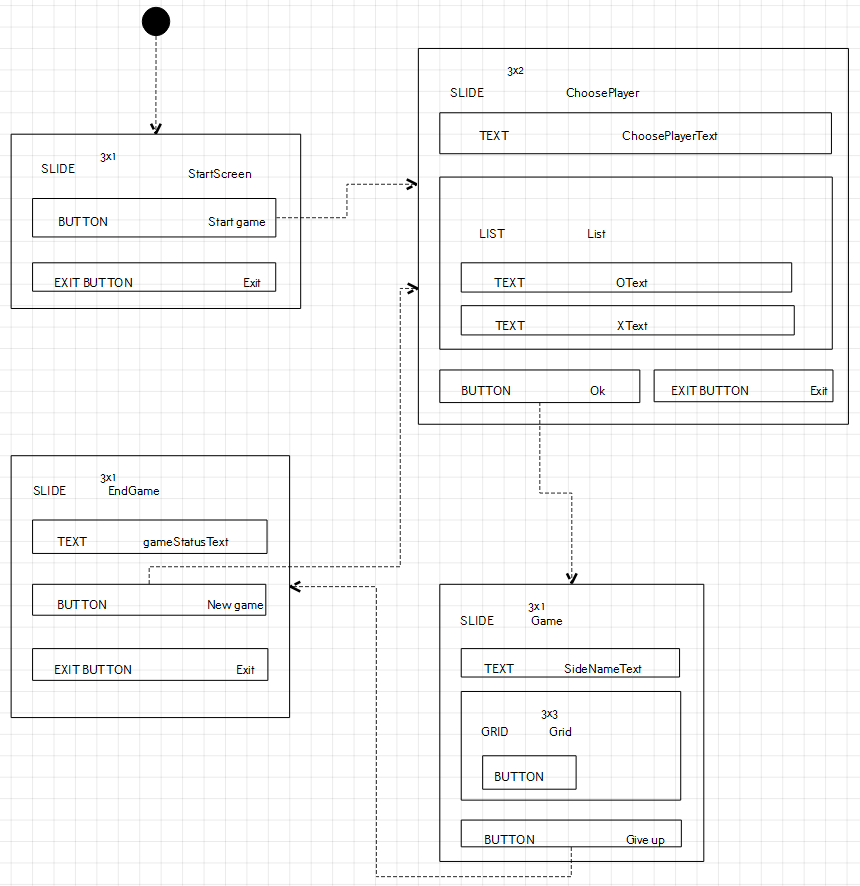
\includegraphics[width=0.9\textwidth]{appendixA/A.2/screenflow.png}
		\caption{Задание интерфейса приложения и переходов между экранами в QReal:Ubiq.}
		\label{image:screenflow}
	\end{center}
\end{figure}

Результатом реализации модельного примера (в качестве которого была выбрана игра <<Крестики-нолики>>) 
стало то, что диаграммы переходов между формами оказались полезны сами по себе, поскольку 
хорошо визуализируют переходы, которые могут быть неочевидны в коде. Кроме того, по 
ним просто сгенерировать скелет приложения, а если сложная логика не требуется (например, 
приложение-визитка), то и приложение целиком. Однако задание сложной логики без кода 
на целевом языке привело к ещё более громоздким диаграммам, которые хоть и проще для 
понимания, чем диаграммы из прототипа, полученного на первом этапе работы, но всё 
же менее удобны, чем ручное кодирование.

\subsection{Результаты проекта QReal:Ubiq}
Первый этап проекта разрабатывался для мастер-класса в рамках конференции FRUCT 2011%
\footnote{Программа FRUCT 2011, URL: http://fruct.org/node/5016 (дата обращения 08.02.2015)}, 
где был успешно продемонстрирован, а на самой конференции был сделан доклад~\cite{bryksin2011ubiq}. 
На мастер-классе демонстрировалась разработка приложения для отображения данных 
с веб-камеры, аудитории был показан процесс создания и генерации логики клиентской 
части. Технология показалась весьма привлекательной авторам Ubiq Mobile, поэтому работа 
над ней была продолжена и после выступления.

С точки зрения исследования визуальных языков результаты проекта оказались менее однозначными: 
конечного ответа на вопрос <<возможно ли эффективно использовать визуальные языки 
вместо текстовых при решении достаточно общих задач>> получено не было. С одной стороны, 
визуальная технология дала очевидный выигрыш в том, что уменьшила объём необходимых 
для программирования знаний, с другой стороны, для некоторых задач, возникающих при 
разработке мобильного приложения, использование текстовых языков пока эффективнее. 

Работа над этим проектом поставила новые вопросы, требующие исследования. 
\begin{enumerate}
	\item Полноценная реализация редактора пользовательского интерфейса с визуализацией 
		переходов между формами (или экранами) средствами \ac{DSM}-платформы. Для этого различные 
		элементы пользовательского интерфейса, такие как поля ввода, кнопки, выпадающие 
		списки и т.д. должны быть полноправными частями формы элемента языка.
	\item Поддержка работы с семействами визуальных языков, каждый из которых может 
		уточнять более общий язык под конкретную задачу. Таким образом может быть реализована 
		схема с настраиваемыми элементами из раздела~\ref{chapter:advancedQRealUbiq} --- 
		создать общий язык разработки мобильных приложений, от него породить язык задания 
		игр с полем, от него --- язык, содержащий специфические блоки для игры <<Морской бой>>. 
		Это не снимает всех проблем, перечисленных в разделе~\ref{chapter:advancedQRealUbiq} 
		касательно этой схемы, но представляется логичным развитием идей \ac{DSM}-подхода.
\end{enumerate}